%\documentclass[UTF8]{ctexart} % use larger type; default would be 10pt
\documentclass[a4paper]{article}
\usepackage{xeCJK}
%\usepackage[utf8]{inputenc} % set input encoding (not needed with XeLaTeX)

%%% Examples of Article customizations
% These packages are optional, depending whether you want the features they provide.
% See the LaTeX Companion or other references for full information.

%%% PAGE DIMENSIONS
\usepackage{geometry} % to change the page dimensions
\geometry{a4paper} % or letterpaper (US) or a5paper or....
\geometry{margin=1in} % for example, change the margins to 2 inches all round
% \geometry{landscape} % set up the page for landscape
%   read geometry.pdf for detailed page layout information

\usepackage{graphicx} % support the \includegraphics command and options

% \usepackage[parfill]{parskip} % Activate to begin paragraphs with an empty line rather than an indent

%%% PACKAGES
\usepackage{booktabs} % for much better looking tables
\usepackage{array} % for better arrays (eg matrices) in maths
\usepackage{paralist} % very flexible & customisable lists (eg. enumerate/itemize, etc.)
\usepackage{verbatim} % adds environment for commenting out blocks of text & for better verbatim
\usepackage{subfig} % make it possible to include more than one captioned figure/table in a single float
% These packages are all incorporated in the memoir class to one degree or another...

%%% HEADERS & FOOTERS
\usepackage{fancyhdr} % This should be set AFTER setting up the page geometry
\pagestyle{fancy} % options: empty , plain , fancy
\renewcommand{\headrulewidth}{0pt} % customise the layout...
\lhead{}\chead{}\rhead{}
\lfoot{}\cfoot{\thepage}\rfoot{}

%%% SECTION TITLE APPEARANCE
\usepackage{sectsty}
%\allsectionsfont{\sffamily\mdseries\upshape} % (See the fntguide.pdf for font help)
% (This matches ConTeXt defaults)

%%% ToC (table of contents) APPEARANCE
\usepackage[nottoc,notlof,notlot]{tocbibind} % Put the bibliography in the ToC
\usepackage[titles,subfigure]{tocloft} % Alter the style of the Table of Contents
%\renewcommand{\cftsecfont}{\rmfamily\mdseries\upshape}
%\renewcommand{\cftsecpagefont}{\rmfamily\mdseries\upshape} % No bold!

%%% END Article customizations

%%% The "real" document content comes below...

\setlength{\parindent}{0pt}
\usepackage{physics}
\usepackage{amsmath}
%\usepackage{symbols}
\usepackage{AMSFonts}
\usepackage{bm}
%\usepackage{eucal}
\usepackage{mathrsfs}
\usepackage{amssymb}
\usepackage{float}
\usepackage{multicol}
\usepackage{abstract}
\usepackage{empheq}
\usepackage{extarrows}
\usepackage{textcomp}
\usepackage{fontspec}

\setmainfont{CMU Serif}
\setsansfont{CMU Sans Serif}
\setmonofont{CMU Typewriter Text}

\usepackage{braket}
\usepackage{siunitx}
\sisetup{
	separate-uncertainty = true,
	inter-unit-product = \ensuremath{{}\cdot{}}
}
\usepackage{mhchem}
\usepackage{multirow}
\usepackage{booktabs}
\usepackage[isbn=false,doi=true,url=false,
%uniquename=init,
style=chem-acs]{biblatex}
\addbibresource{hw2.bib}

\DeclareMathOperator{\p}{\prime}
\DeclareMathOperator{\ti}{\times}
\DeclareMathOperator{\intinf}{\int_0^\infty}
\DeclareMathOperator{\intdinf}{\int_{-\infty}^\infty}
\DeclareMathOperator{\intzpi}{\int_0^\pi}
\DeclareMathOperator{\intztpi}{\int_0^{2\pi}}
\DeclareMathOperator{\sumninf}{\sum_{n=1}^{\infty}}
\DeclareMathOperator{\sumninfz}{\sum_{n=0}^\infty}
\DeclareMathOperator{\sumiinf}{\sum_{i=1}^{\infty}}
\DeclareMathOperator{\sumiinfz}{\sum_{i=0}^\infty}
\DeclareMathOperator{\sumkinf}{\sum_{k=1}^{\infty}}
\DeclareMathOperator{\sumkinfz}{\sum_{k=0}^\infty}
\DeclareMathOperator{\e}{\mathrm{e}}
\DeclareMathOperator{\I}{\mathrm{i}}
\DeclareMathOperator{\Arg}{\mathrm{Arg}}
\DeclareMathOperator{\ra}{\rightarrow}
\DeclareMathOperator{\llra}{\longleftrightarrow}
\DeclareMathOperator{\lra}{\longrightarrow}
\DeclareMathOperator{\dlra}{\Leftrightarrow}
\DeclareMathOperator{\dra}{\Rightarrow}
\newcommand{\bkk}[1]{\Braket{#1|#1}}
\newcommand{\bk}[2]{\Braket{#1|#2}}
\newcommand{\bkev}[2]{\Braket{#2|#1|#2}}



\DeclareMathOperator{\hV}{\hat{\vb{V}}}

\DeclareMathOperator{\hx}{\hat{\vb{x}}}
\DeclareMathOperator{\hy}{\hat{\vb{y}}}
\DeclareMathOperator{\hz}{\hat{\vb{z}}}

\DeclareMathOperator{\hA}{\hat{\vb{A}}}

\DeclareMathOperator{\hQ}{\hat{\vb{Q}}}
\DeclareMathOperator{\hI}{\hat{\vb{I}}}
\DeclareMathOperator{\psis}{\psi^\ast}
\DeclareMathOperator{\Psis}{\Psi^\ast}
\DeclareMathOperator{\hi}{\hat{\vb{i}}}
\DeclareMathOperator{\hj}{\hat{\vb{j}}}
\DeclareMathOperator{\hk}{\hat{\vb{k}}}
\DeclareMathOperator{\hr}{\hat{\vb{r}}}
\DeclareMathOperator{\hT}{\hat{\vb{T}}}
\DeclareMathOperator{\hH}{\hat{H}}
\DeclareMathOperator{\hh}{\hat{h}}               % helicity
\DeclareMathOperator{\hL}{\hat{\vb{L}}}
\DeclareMathOperator{\hp}{\hat{\vb{p}}}

\DeclareMathOperator{\ha}{\hat{\vb{a}}}
\DeclareMathOperator{\hs}{\hat{\vb{s}}}
\DeclareMathOperator{\hS}{\hat{\vb{S}}}
\DeclareMathOperator{\hSigma}{\hat{\bm\Sigma}}
\DeclareMathOperator{\hJ}{\hat{\vb{J}}}
\DeclareMathOperator{\hP}{\hat{\vb{P}}}          % Parity
\DeclareMathOperator{\hC}{\hat{\vb{C}}} 
\DeclareMathOperator{\Tdv}{-\dfrac{\hbar^2}{2m}\dv[2]{x}}
\DeclareMathOperator{\Tna}{-\dfrac{\hbar^2}{2m}\nabla^2}
\DeclareMathOperator{\vna}{\vnabla}
\DeclareMathOperator{\nna}{\nabla^2}
\newcommand{\naCarExpd}[1]{\pdv[2]{#1}{x} + \pdv[2]{#1}{y} + \pdv[2]{#1}{z}}
\newcommand{\naCyl}{\qty[\dfrac{1}{\rho}\pdv{\rho}\qty(\rho\pdv{\rho}) + \dfrac{1}{\rho^2}\pdv[2]{\phi} + \pdv[2]{z}]}

%\DeclareMathOperator{\g#0}{\gamma^0}
%\DeclareMathOperator{\g1}{\gamma^1}
%\DeclareMathOperator{\g2}{\gamma^2}
%\DeclareMathOperator{\g3}{\gamma^3}
%\DeclareMathOperator{\g5}{\gamma^5}
\newcommand{\g}[1]{\gamma^{#1}}
\DeclareMathOperator{\gmuu}{\gamma^\mu}
\DeclareMathOperator{\gmud}{\gamma_\mu}
\newcommand{\G}[2]{g^{#1#2}}


%% MQC
\DeclareMathOperator{\sH}{\mathscr{H}}
\DeclareMathOperator{\sA}{\mathscr{A}}
\newcommand{\iden}{{\large \bm{1}}}
\newcommand{\qed}{$ \Square $}
\newcommand{\tPhi}{\tilde{\Phi} }
\newcommand{\hsP}{\hat{\mathscr{P}}}
\newcommand{\hsS}{\hat{\mathscr{S}}}
\DeclareMathOperator{\core}{\mathrm{core}}
\DeclareMathOperator{\GF}{\mathrm{GF}}
\DeclareMathOperator{\SF}{\mathrm{SF}}
\DeclareMathOperator{\corr}{\mathrm{corr}}
\DeclareMathOperator{\gvb}{\mathrm{GVB}}


\newcommand{\subsbul}{\subsection*{$ \bullet $}}
\newcommand{\ex}[1]{\paragraph{Ex #1}}
\newcommand{\subex}[1]{\subparagraph{#1}}
\newcommand{\dis}{\displaystyle}


\numberwithin{equation}{subsection}
%\setcounter{secnumdepth}{4}
\setcounter{tocdepth}{4}
\allowdisplaybreaks[1]

\usepackage{xcolor}
\definecolor{codegray}{gray}{0.9}
\newfontfamily\Consolas{Consolas}
\newcommand{\code}[1]{\colorbox{codegray}{{\Consolas#1}}}

\title{\textbf{Theoretical and Physical Organic Chemistry}\\Homework II}
\author{王石嵘
\vspace{5pt}\\
161240065\\
Kuang Yaming Honors School
%Email: shirong\_wang@berkeley.edu
}
\date{\today} % Activate to display a given date or no date (if empty),
         % otherwise the current date is printed 

\begin{document}
\maketitle
% \boldmath
\section{}
\subsection*{A.}
$ S_N $I reaction with Lucas reagent (last step)\\
\begin{figure}[H]
	\centering
	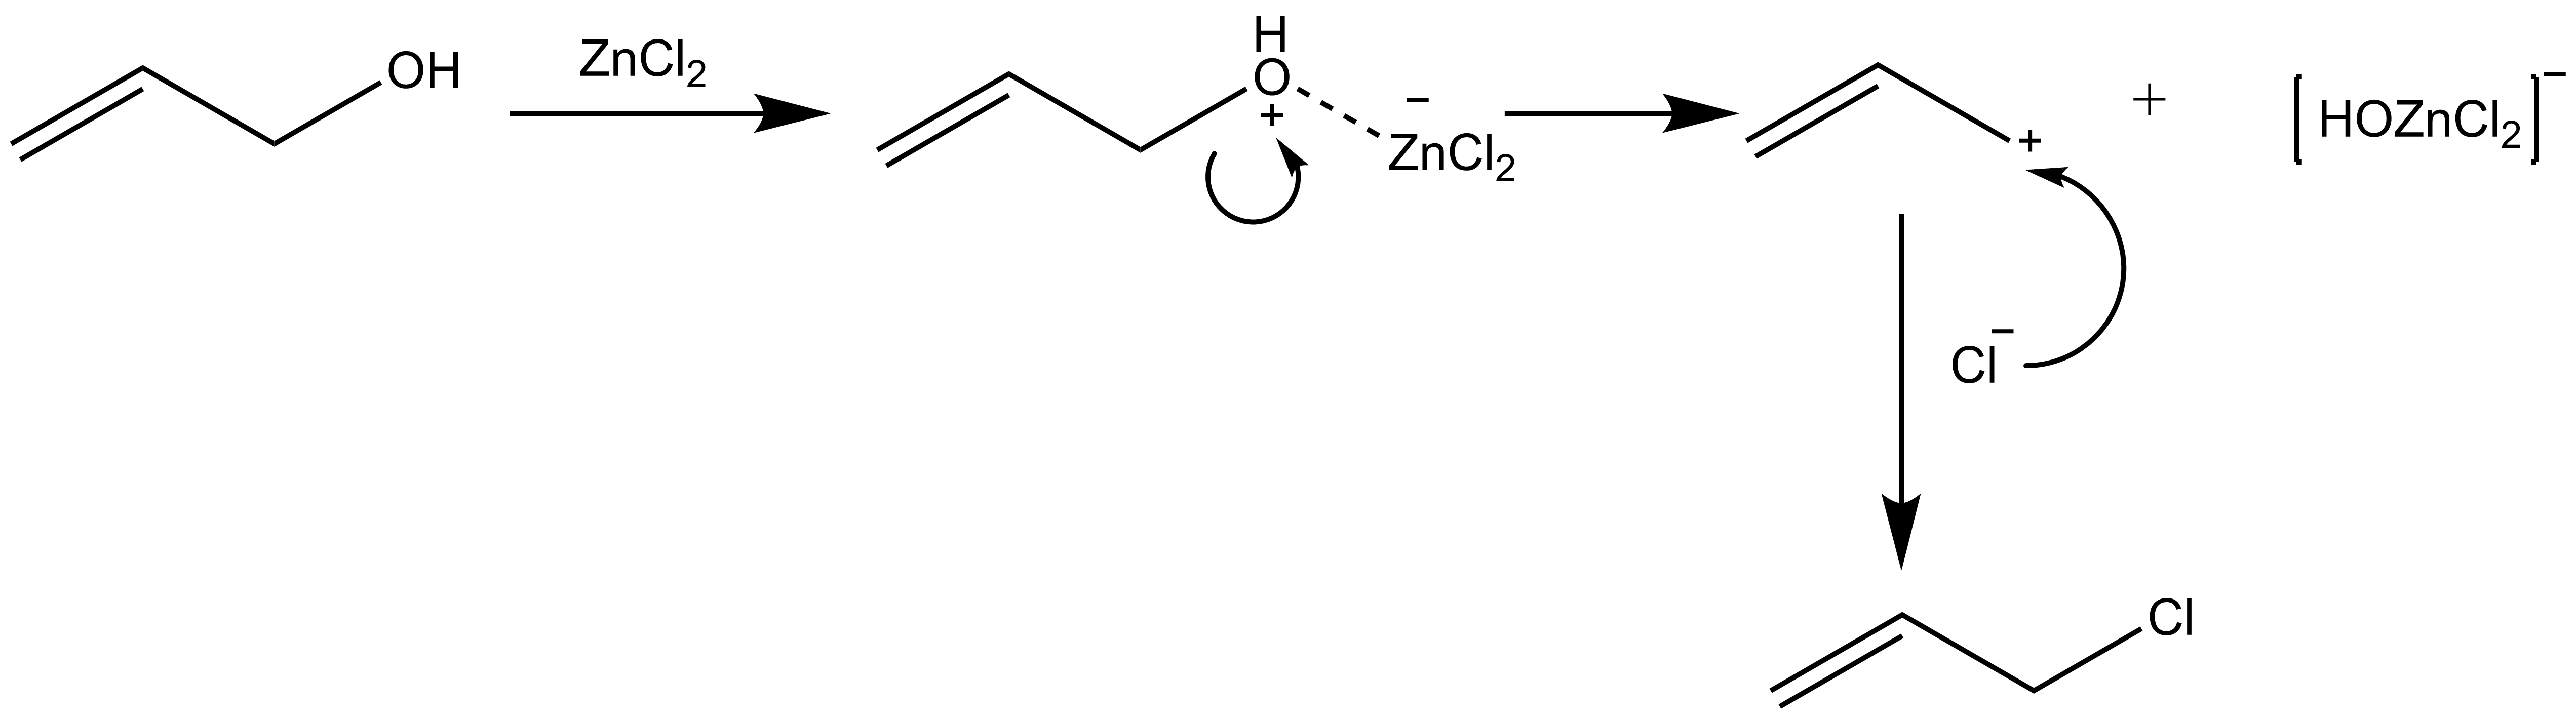
\includegraphics[width=0.9\linewidth]{lucas.png}
\end{figure}
%~\vspace{10pt}\\
%\hfill\fullcite{bateman} 
\hfill\fullcite{lucas}

\subsection*{B.}
pinacol rearrangement (last step)
\begin{figure}[H]
	\centering
	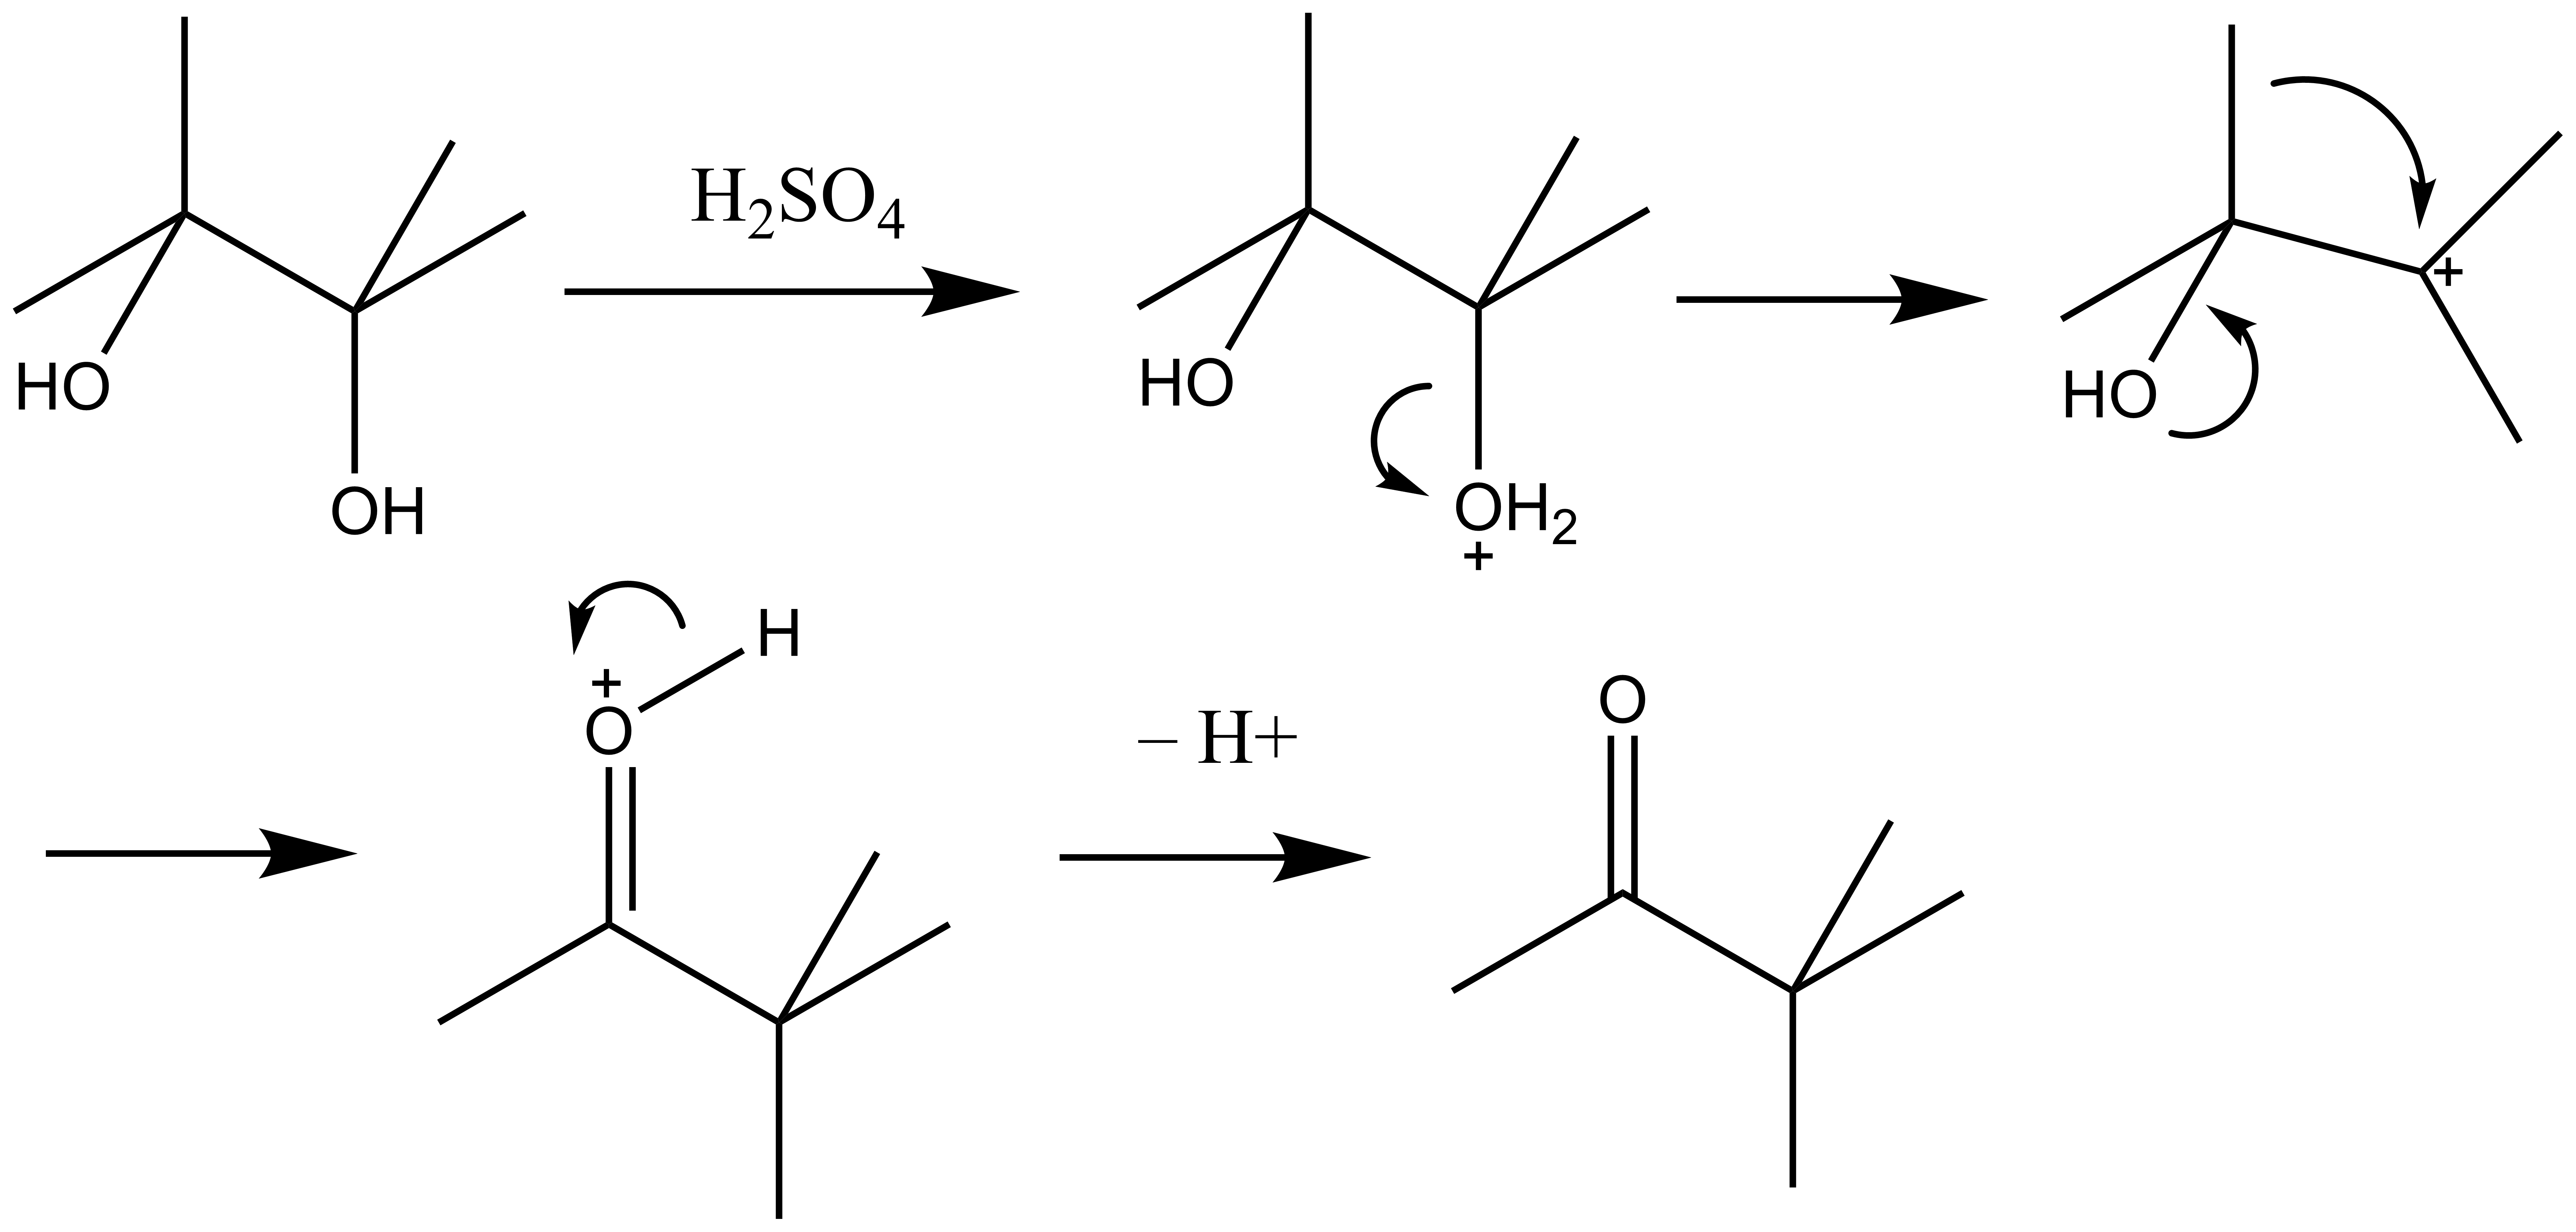
\includegraphics[width=0.75\linewidth]{pinacol.png}
\end{figure}
%~\vspace{10pt}\\
\hfill\fullcite{fittig}

\subsection*{C.}
Wagner-Meerwein rearrangement
\begin{figure}[H]
	\centering
	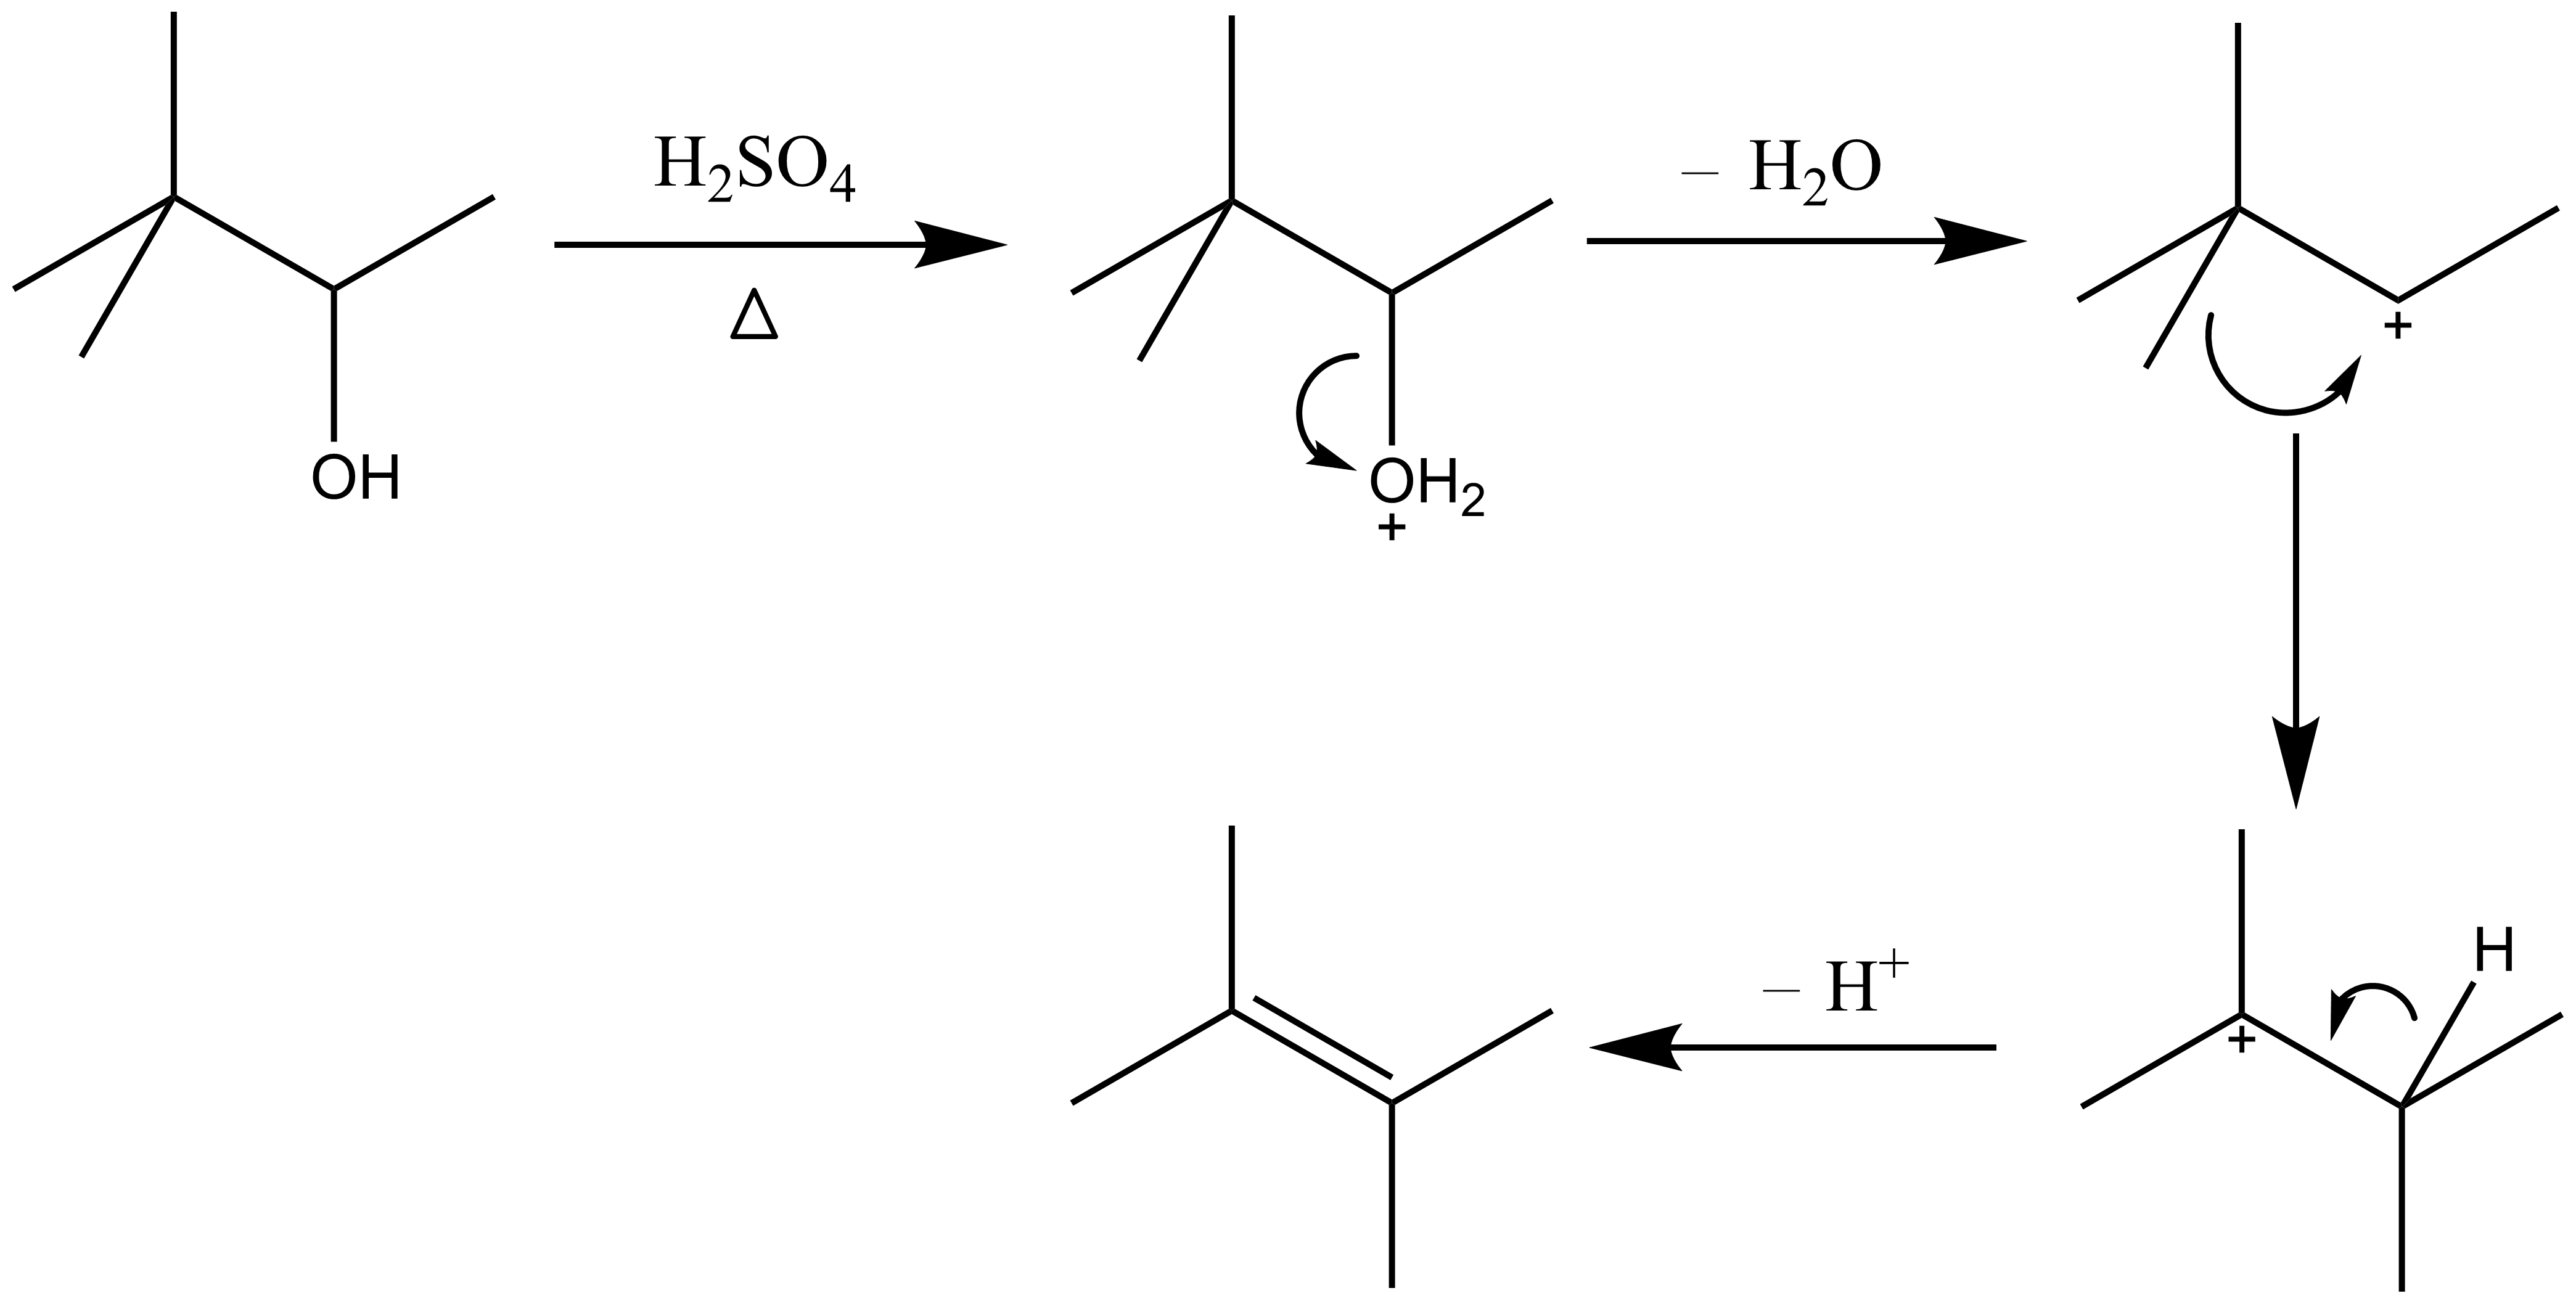
\includegraphics[width=0.75\linewidth]{wagner.png}
\end{figure}

%~\vspace{10pt}\\
\subsection*{D.}
Prins reaction
\begin{figure}[H]
	\centering
	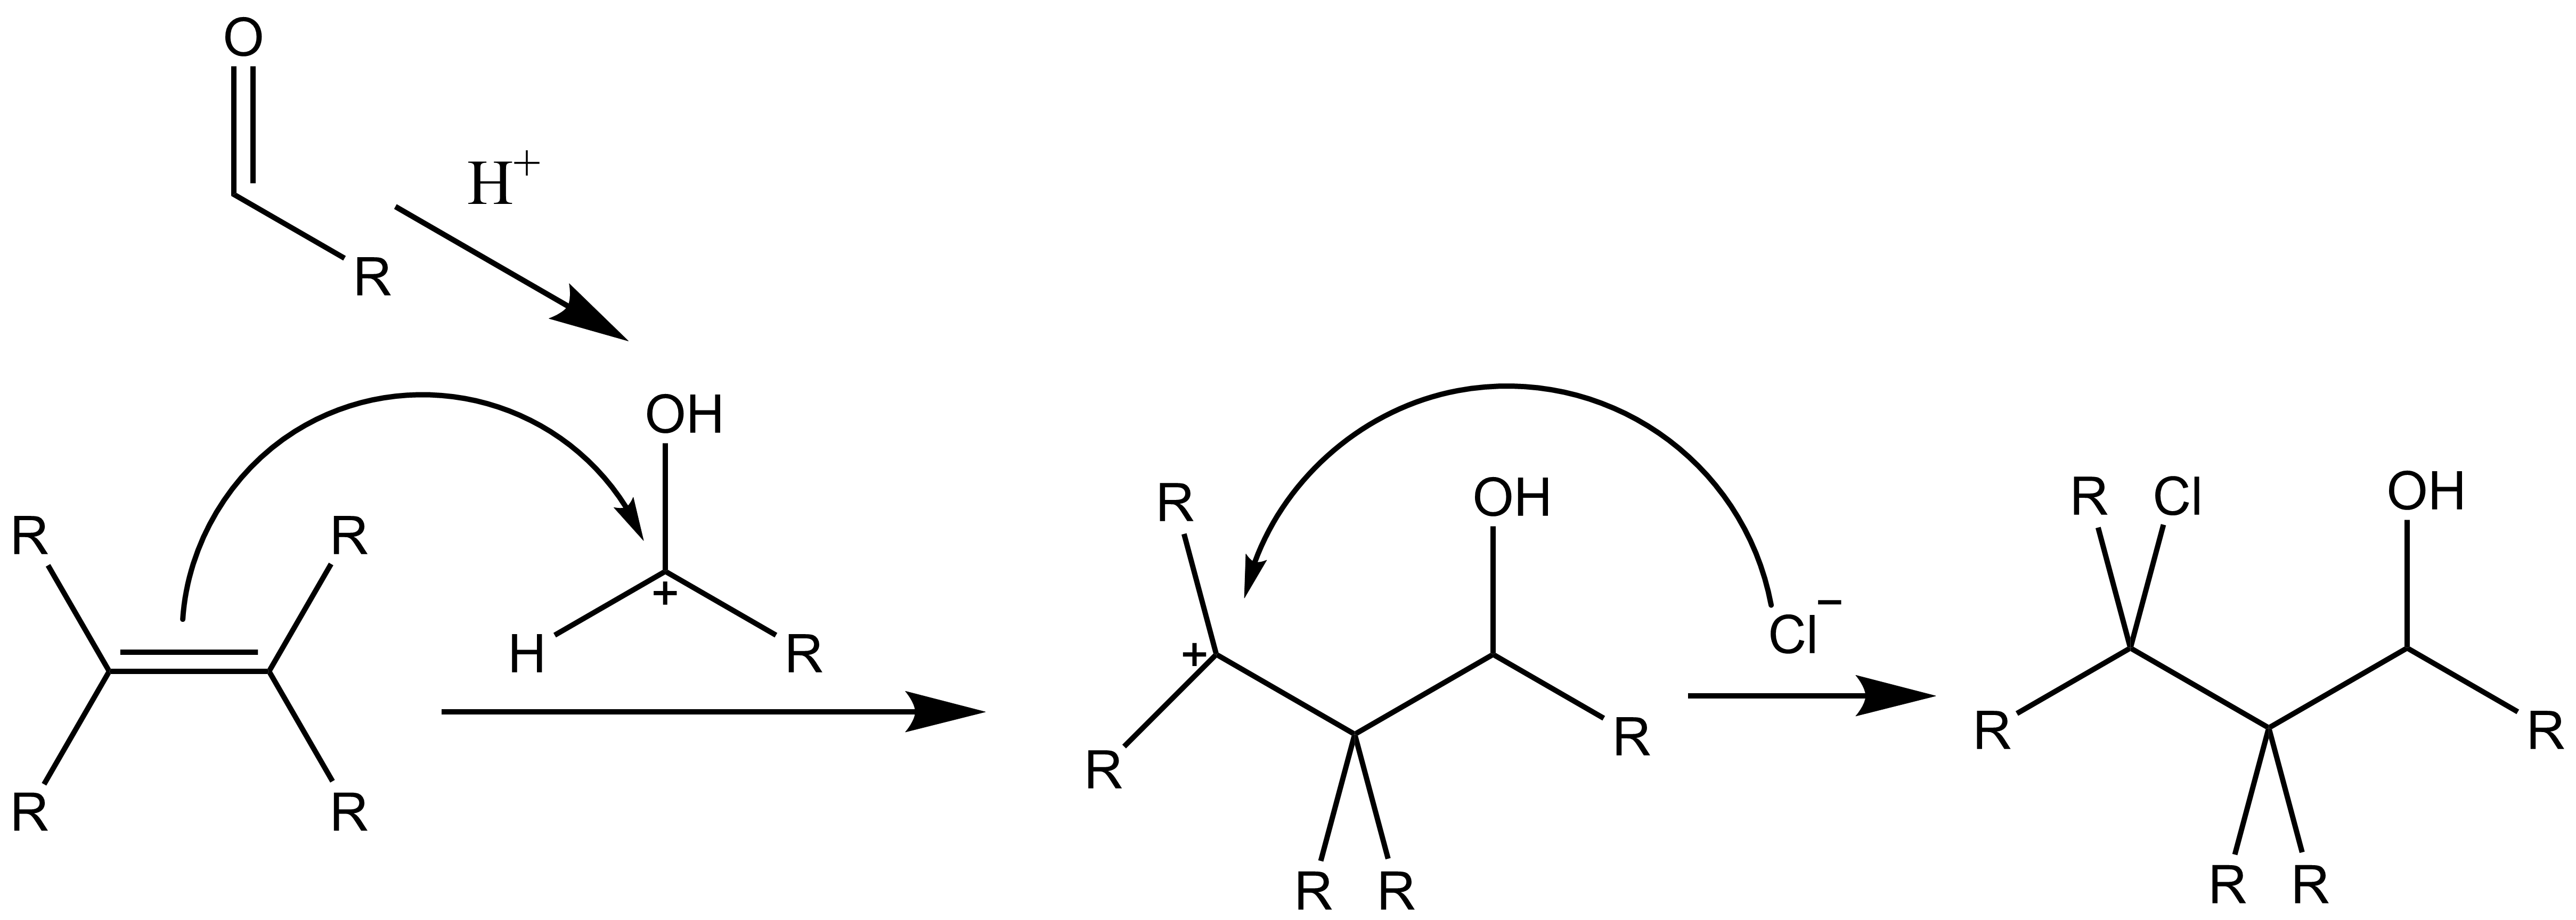
\includegraphics[width=0.8\linewidth]{prins.png}
\end{figure}

\newpage
\section{}
\subsection*{A. Generation of Halomethyl Radicals by Halogen Atom Abstraction and Their Addition Reactions with Alkenes}
\begin{figure}[H]
	\centering
	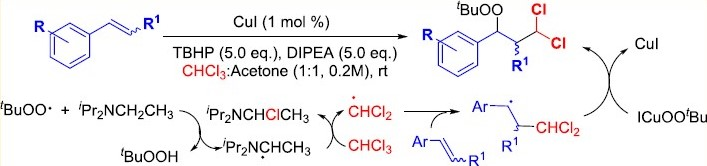
\includegraphics[width=0.9\linewidth]{neff.jpg}
\end{figure}
\hfill\fullcite{neff}\\
\paragraph{Generation of radicals}~\\
Using $ t\textendash\ce{BuOO}\cdot $ to generate $ \cdot\ce{CHCl_2} $, where $ t\textendash\ce{BuOO}\cdot $ is generated by the reaction of $ t\textendash\ce{BuOOH} $(TBHP) and $ \ce{CuI} $.\\
\paragraph{Proof of the radical mechanism}
\begin{itemize}
	\item TEMPO trapping experiment
	\begin{figure}[H]
		\centering
		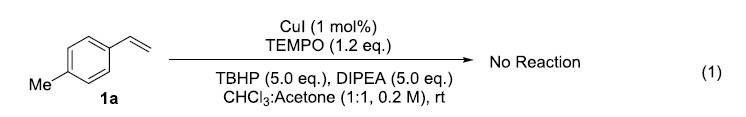
\includegraphics[width=0.9\linewidth]{neff-mech.jpg}
	\end{figure}
	\item Mechanistic experiment with vinylcyclopropane
\begin{figure}[H]
	\centering
	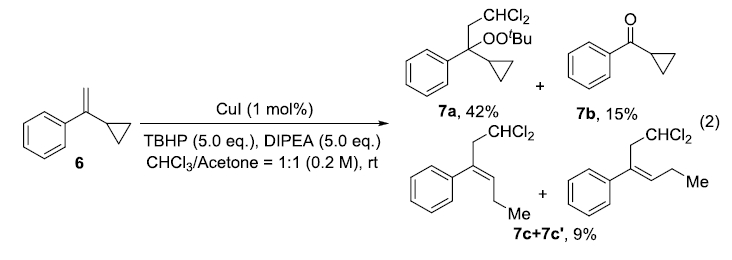
\includegraphics[width=0.9\linewidth]{neff-mech2.jpg}
\end{figure}
\end{itemize}

\newpage
\subsection*{B. Catalyzing the Hydrodefluorination of \ce{ CF_3}‑Substituted Alkenes by \ce{PhSiH_3}. \ce{H}$\cdot $ Transfer from a Nickel Hydride}
\begin{figure}[H]
	\centering
	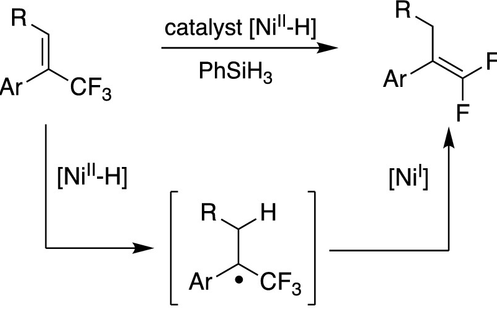
\includegraphics[width=0.5\linewidth]{yao.png}
\end{figure}
\hfill\fullcite{yao}\\
\paragraph{Generation of radicals}~\\
	\begin{figure}[H]
	\centering
	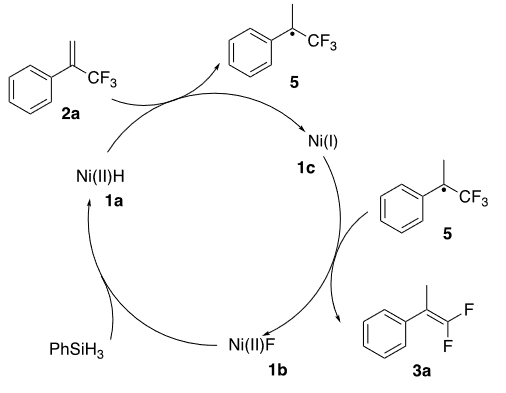
\includegraphics[width=0.6\linewidth]{yao-mech.jpg}
\end{figure}
Radical is initiated by $ \ce{H}\cdot $ transfer from nickel hydride.\\
\paragraph{Proof of the radical mechanism}~\\
	\begin{figure}[H]
	\centering
	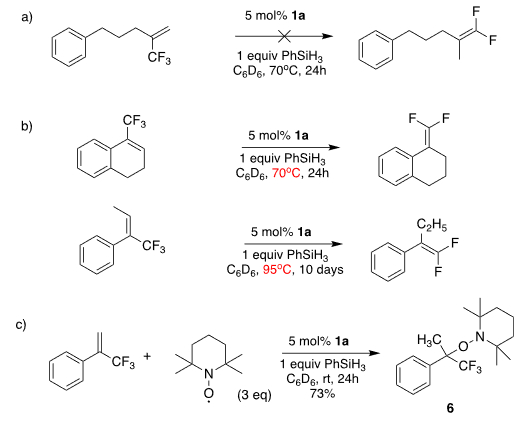
\includegraphics[width=0.9\linewidth]{yao-mech2.jpg}
\end{figure}
\begin{itemize}
	\item a) Aliphatic alkenes do not work even at an elevated temperature. Aryl group is essential for stabilizing the organic radical resulting from HAT (Hydrogen Atom Transfer), compared with another possible mechanism (Fluorine Atom Abstraction).
	\item b) Methyl substituent on the carbon receiving the $ \ce{H}\cdot $(in the second mechanism) is known to slow HAT, while should not affect another mechanism.
	\item c) TEMPO trapping experiment

\end{itemize}


\end{document}